\chapter{Renormalización}
\label{ch:renormalizacion}

El propósito de toda teoría física es calcular cantidades medibles y observables en el mundo real. En el formalismo de las teorías de campos aparecen elementos matemáticos que representan cantidades física, pero también otros que no tienen un paralelo directo en el mundo real, sino que son cantidades puramente abstractas que sólo existen como parte del aparato matemático.

Ejemplo de ello es la denominada \emph{masa desnuda}, una cantidad teórica asociada al parámetro de masa en el Lagrangiano. Dicho término de masa siempre es proporcional al campo al cuadrado y aparece para todas las partículas de la teoría. En el caso del modelo estándar, dicho parámetro de masa aparece incluso en el caso de los quarks, aún cuando éstos no tienen masa física.

La esencia de la \textbf{renormalización} en teoría cuántica de campos consiste en conectar estas cantidades abstractas -- denominadas prámetros desnudos -- que aparecen en el Lagrangiano, a cantidades medibles y observables. 

En general toda teoría, bien sea clásica o bien sea cuántica, requiere de un proceso de renormalización. No obstante, la necesidad de renormalizar una teoría nunca fue tan evidente como en el cálculo de cantidades a un loop en teoría cuántica de campos, realizados por primera vez durante la década de 1930. Como ya mencionamos en el capítulo \ref{ch:anomalias}, las amplitudes de diagramas a un loop suelen resultar en infinitos. Recordemos que cuando dichos diagramas corresponden a procesos que no existen en el Lagrangiano, representan una anomalía cuántica, cuya cancelación hace que la teoría siga siendo consistente.


No obstante, otros procesos que sí son posibles a nivel árbol resultan en infinitos ineludibles cuando se calculan a un loop. Estos infinitos son denominados \textbf{divergencias ultravioletas}. El proceso de renormalización es crucial para que dichos cálculos tengan sentido físico y permite una definición unívoca de los parámetros desnudos.

\section{Grado superficial de divergencia}

Es importante identificar qué diagramas originan divergencias y en qué teorías tales divergencias pueden ser eliminadas sistemáticamente. En esta sección emplearemos argumetos elementales para determinar, tentativamente, qué diagramas de Feynman contienen una divergencia ultravioleta. Iniciamos analizando el caso de la QED, partiendo de algunas definiciones:


\begin{definition}
\begin{equation*}
	\begin{IEEEeqnarraybox}[][c]{rCl}
		N_e &=& \text{número de lineas externas asociadas al electrón,} \\
		%%%%
		N_\gamma &=& \text{número de lineas externas asociadas al fotón,} \\
		%%%%
		P_e &=& \text{número de propagadores del electrón,} \\
		%%%%
		P_\gamma &=& \text{número de propagadores del fotón,} \\
		%%%%
		V &=& \text{número de vértices,} \\
		%%%%
		L &=& \text{número de loops,} \\
		%%%%
		D &=& \text{grado superficial de divergencia.}
	\end{IEEEeqnarraybox}
\end{equation*}
\end{definition}

Este concepto de grado superficial de divergencia no será útil para todos los diagramas, pero será importante, en particular, para una clase de diagramas que denominaremos \emph{diagramas irreducibles de una partícula} (one-particle irreducible). Para entender este concepto, primero definamos lo que es un diagrama irreducible. \\

\begin{definition}[Diagrama irreducible de $n$ partículas]
	Un \emph{diagrama de $n$ partículas} es aquel en el que entran $n$ partículas y salen $n$ partículas. El diagrama es \textbf{irreducible} si, mediante $n$ cortes en las líneas internas, no es posible reducirlo a otros diagramas de $n$ partículas.
\end{definition} 

 Como ejemplo, consideremos el diagrama en la Figura~\ref{fig:1partredu_ladder}, conocido como diagrama escalera (ladder). Si cortamos dos de las lineas internas del diagrama por los puntos indicados, obtenemos dos diagramas que son también de dos partículas. Esto es, el diagrama escalera de dos partículas inicial \emph{es reducible}.

\begin{figure}[ht]
	\centering
	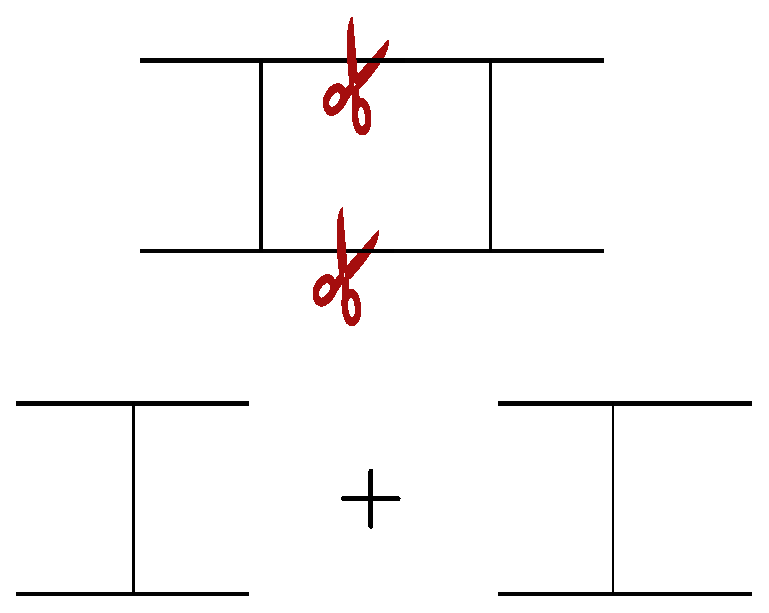
\includegraphics[scale=0.3]{Pictures/1partRedu_ladder.eps}
	\caption{Un diagrama escalera de dos partículas que se corta por los puntos indicados se convierte en dos diagramas de dos partículas, por lo tanto el diagrama inicial es reducible.}
	\label{fig:1partredu_ladder}
\end{figure}

Ahora, consideremos el caso en la Figura~\ref{fig:1parirred_mount}, donde tenemos un diagrama de una sola partícula que emite un fotón y lo reabsorbe. Al realizar un solo corte (pues el diagrama es de una partícula) por una linea interna, ya no obtenemos un diagrama de una partícula. Incluso podríamos pensar que el diagrama final es de dos partículas, pues tiene dos patas externas. Este diagrama, por consiguiente, \emph{es un diagrama irreducible de una partícula}.

\begin{figure}[ht]
	\centering
	
\includegraphics[scale=0.2]{1partIrred_mount.eps}
	\caption{Un diagrama de una partícula con un fotón que es emitido y reabsorbido. Al cortar por la línea indicada no se obtiene un diagrama de una partícula, por lo que este es un diagrama irreducible.}
	\label{fig:1parirred_mount}
\end{figure}

La idea general de los diagramas irreducibles es que a partir de ellos se pueden construir diagramas más complejos. Todo diagrama se puede construir a partir de diagramas irreducibles. Son una especie de equivalente de los números primos para el conjunto de los números naturales. Entonces, tengamos en cuenta lo siguiente: 

\begin{cabox}
	El concepto de grado superficial de divergencia será aplicado únicamente a diagramas irreducibles.
\end{cabox}

Con estos fundamentos claros, procedamos ahora a explorar de qué se trata el grado superficial de divergencia.

Típicamente, las expresiones correspondientes a un diagrama típico en QED serán de la forma
%
\begin{IEEEeqnarray}{rCl}
	\int \dd[4]{k_1} \dd[4]{k_2} \cdots \dd[4]{k_L} \frac{1}{\underbrace{(\slashed{k}_i - m)}_{\substack{\text{propagadores} \\ \text{de fermiones}}} \cdots \underbrace{k_j^2 \cdots k_n^2}_{\substack{\text{propagadores} \\ \text{de fotones}}}} 
\end{IEEEeqnarray}

El diagrama que consideramos tendrá tantas integrales en $k$ como loops hayan. Definiremos el grado superficial de divergencia como
%
\begin{equation}
\boxed{
	D = 4L - P_e - 2P_\gamma \,.
}
\end{equation}

Para comprender la el razonamiento detrás de esta expresión, consideremos lo siguiente: sabemos que por cada loop que hay en el diagrama habrá una integral $\dd[4]k_i$. Estamos interesados en la dimensión, en unidades de momento, del integrando. En unidades de momento, cada diferencial tiene dimensión $4$, i.e., cada loop aportará un $4$ a la dimensión del integrando. Ahora, los propagadores fermiónicos son de la forma
%
\begin{equation*}
	\frac{\ii}{\slashed{k} - m} \,,
\end{equation*}

\noindent de modo que, por cada propagador fermiónico la dimensión del integrando, en unidades de momento, disminuye en una unidad. Por su parte, los propagadores de fotones son de la forma
%
\begin{equation*}
	\frac{\ii}{k^2} \,,
\end{equation*}

\noindent haciendo que por cada propagador de fotones la dimensión del integrando, en unidades de momento, disminuya en dos unidades.

El grado superficial de divergencia, como podemos ver, es la dimensión del integrando en unidades de momento. Hablando de manera muy general, un diagrama diverge, a menos que hayan más potencias de momento en el denominador que en el numerador.

En general, podríamos esperar que el diagrama tenga una divergencia proporcional a $\Lambda ^D$, donde $\Lambda$ es un límite superior de los momentos, denominado \emph{corte} o \emph{cutoff}. En este escenario, podemos considerar los siguientes casos:

%
\begin{profor}
    \begin{equation*}
	\begin{IEEEeqnarraybox}[][c]{ll}
		\text{Si } D > 0 \qc & \text{la divergencia es proporcional a } \Lambda^D\,; \\
		%%%%
		\text{si } D = 0 \qc & \text{la divergencia es proporcional a } \log \Lambda \,; \\
		%%%%
		\text{si } D < 0 \qc & \text{las cantidades irań como } \Lambda^{-D} \text{ y son típicamente convergentes.}
	\end{IEEEeqnarraybox}
\end{equation*}
\end{profor}

Cabe anotar que esto no es una regla general. Existen diagramas que pueden contener divergencias no contempladas en este análisis, o diagramas convergentes cuyo grado superficial de divergencia puede ser igual a cero. No obstante, las condiciones dadas arriba se cumplen en muchos casos para los diagramas irreducibles.

Ahora, en QED el número de loops es dado por
%
\begin{equation}
	L = P_e + P_\gamma - \qty(V - 1) \,.
\end{equation}

Esto proviene de las reglas de Feynman, que exigen que por cada propagador debe haber una integral~\footnote{cf. David Griffiths. \emph{Introduction to Elementary Particles}. Second Edition. Wiley-VCH, 2008. Capítulos 6 y 7.}. No obstante, por cada vértice debe haber una delta de Dirac, que eliminará una de las integrales. Ahora, una de las deltas de Dirac expresará la conservación global del momento lineal, y esta delta no se integraba como las demás. A esta delta que no va a eliminar una integral se debe el $-1$ en el paréntesis. Finalmente, el número de loops es el número de integrales de cuatro dimensiones presentes en la expresión.

Para el número de vértices tenemos la expresión
%
\begin{equation}
	V = 2P_\gamma + N_\gamma \,,
\end{equation}

\noindent que se sigue de la estructura del vértice fundamental de QED, que siempre involucra un fotón. Si el fotón está como línea interna, debe estar asociado a dos vértices, mientras que si es una pata externa, estará asociado a uno solo. También es posible expresar el número de vértices como
%
\begin{equation}
	V = P_e + \frac{N_e}{2}\,,
\end{equation}

\noindent lo cual también responde a la estructura del vértice fundamental de QED.

Con estas expresiones podemos escribir el grado de divergencia como
%
\begin{IEEEeqnarray*}{rCl}
	D &=& 4L - P_e - 2\gamma \\
	%%%%
	&=& 4 \qty(P_e + P_\gamma - V + 1) - P_e - 2P_\gamma \\
	%%%%
	&=& 4 + 4P_\gamma + \cancel{4P_e} - 4 \qty(\cancel{P_e} + \frac{N_e}{2}) - P_e - 2P_\gamma \\
	%%%
	&=& 4 + 2P_\gamma - 2N_e - P_e \\
	%%%%
	&=& 4 + \cancel{2P_\gamma} - 2N_e - \qty(\cancel{2P_\gamma} + N_\gamma - frac{N_e}{2}) \\
	%%%%
	&=& 4 - 2N_e + \frac{N}{2} - N-\gamma \slj
	%%%%
	\IEEEeqnarraymulticol{3}{c}{\boxed{ D = 4 - \frac{3}{2}N_e - N_\gamma }\,. \IEEEyesnumber}
\end{IEEEeqnarray*}

Notemos que este resultado no depende de los propagadores, sino únicamente de las patas externas. \\


Para el caso de una teoría $\lambda \phi^n$, i.e. de la forma
%
\begin{equation}
	\lagdn = \frac{1}{2} (\partial_\mu \phi)(\partial^\mu \phi) - \frac{1}{2} m\phi^2 - \frac{\lambda}{n!} \phi^n \,,
\end{equation}

\noindent el número de loops será
%
\begin{equation}
	L = P - V + 1 \qc nV = N + 2P \,,
\end{equation}

\noindent puesto que sólo tenemos una partícula, y por lo tanto sólo tenemos propagadores y patas externas de una misma naturaleza. También se cumple que el grado de divergencia
%
\begin{equation}
	D = dL - 2P \,,
\end{equation}

\noindent donde $d$ es la dimensión de las integrales de momento, que en el caso de QED era 4, pero en este caso es arbitraria. Es posible mostrar que~\footnote{cf. Michael E. Peskin, Daniel V. Schroeder. \emph{An Introduction to Quantum Field Theory}. Addison-Wesley, 1995. Capítulo 10.}
%
\begin{equation}
	D = d + \qty[n \qty(\frac{d-2}{2}) - d]V - \frac{d-2}{2}N \,.
\end{equation} \\


Ahora, recordemos un poco las dimensiones que tienen algunas cantidades en unidades naturales. Al definir unidades naturales se tiene que la constante de Planck $h = 1$, es decir tiene dimensión cero en unidades naturales. Como $h$ tiene unidades de acción, esto hace que la acción tenga dimensión cero en unidades naturales, $[S] = 0$, y como
%
\begin{equation*}
	S = \int \dd[4]{x} \lagdn \,,
\end{equation*}

\noindent la dimensión del Lagrangiano es $-4$,
%
\begin{equation*}
	[\lagdn] = -4 \,,
\end{equation*}

Recordemos también cómo se define el momento lineal
%
\begin{equation*}
	\vb*{p} = m \vb*{v} \,.
\end{equation*}

Las velocidades son adimensionales en unidades naturales, en virtud de que $v = \dd x / \dd t$, y en unidades naturales la distancia y el tiempo tienen las mismas unidades, ya que $c = 1$. Esto implica que $ct = x$ y que el momento tenga unidades de masa.

Ahora, el momento angular
%
\begin{equation*}
	\vb*{L} = \vb*{x} \cross \vb*{p}
\end{equation*}

\noindent es adimensional, por lo que las $x$ deben tener unidades de $p^{-1}$. Volviendo a la acción, vemos entonces que el diferencial $\dd[4]x$ tiene magnitud $-4$ en unidades de momento, por lo que la densidad lagrangiana, en unidades de momento tiene magnitud
%
\begin{equation}
	[\lagdn] = 4 \qc \text{ en unidades de momento.}
\end{equation}

Consideremos la densidad lagrangiana como la diferencia entre una densidad de energía cinética y una densidad de potencial, $\lagdn = \mathcal{T} - \mathcal{V}$, y consideremos un potencial de la forma
%
\begin{equation}
	V = \sum_{n = 1}^{\infty} \frac{G_n}{n!} \phi^n \,,
\end{equation}

\noindent donde $G_n$ son constantes de acoplamiento.

Como $[\lagdn] = 4$ y el Lagrangiano contiene el término $-m^2 \phi^2$, cuya magnitud debe ser también 4, considerando que $[m] = 1$, tenemos que $[\phi] = 1$. Así pues, para el término en el potencial 
%
\begin{equation}
	\qty[\frac{G_4}{4!} \phi^4] = [G_4]4 = 4\,,
\end{equation}

\noindent de modo que el acoplamiento $G_4$ debe ser adimensional. Entonces, lo que tenemos para las unidades de los acoplamientos es que
%
\begin{equation}
	[G_n] = 4 - n \,.
\end{equation}

Vamos a clasificar los Lagrangianos según el siguiente criterio que enunciamos sin explicación, por el momento:
%
\begin{profor}
\begin{equation*}
	\begin{IEEEeqnarraybox}[][c]{ll}
		\text{si } [G_n] > 0 \qc & \text{decimos que la teoría es \emph{super-renormalizable;}} \\
		%%%%
		\text{si } [G_n] = 0 \qc & \text{decimos que la teoría es \emph{renormalizable;}} \\
		%%%%
		\text{si } [G_n] < 0 \qc & \text{decimos que la teoría es \emph{no-renormalizable.}}  
	\end{IEEEeqnarraybox}
\end{equation*}
\end{profor}

La idea, en general, será que las teorías que incluyen términos con potencias menores o iguales que $4$ tendrán buenas propiedades bajo normalización, mientras que aquellas que incluyan términos con potencias mayores que $4$ presentarán complicaciones para su normalización. 

En el caso de los fermiones, tenemos que en la ecuación de Dirac aparece el término $-m\overline{\psi} \psi$ , que debe tener dimensión 4, de modo que
%
\begin{IEEEeqnarray}{rCl}
	\left[-m \overline{\psi} \psi \right] &=& 4 \\
	%%%%
	1 + 2[\psi] &=& 4 \\
	%%%%
	\therefore [\psi] &=& \frac{3}{2} \,.
\end{IEEEeqnarray}


Por ejemplo, consideremos el Lagrangiano de Fermi
%
\begin{equation}
	\lagdn = G_F J_\mu J^\mu \,,
\end{equation}

\noindent donde
%
\begin{equation}
	J_\mu = \overline{\psi} \gamma^\mu \psi \quad \therefore \quad [J_\mu] = 3 \,,
\end{equation}

\noindent de modo que el operador $J_\mu J^\mu$ tiene dimensión 6, con lo cual
%
\begin{equation}
	[G_F] = -2\,,
\end{equation}

\noindent la teoría de Fermi es no-renormalizable.


Estas denominaciones para los Lagrangianos son mencionadas aquí sin más, a manera de definiciones. La justificación para ellas es complicada y la desarrollaremos a medida que veamos los ejemplos particulares en este capítulo.




%------------------------------------------------------
\section{Teoría de perturbación renormalizada}

Ahora, para obtener expresiones que resulten en amplitudes finitas, aún cuando tratemos con diagramas divergentes, el Lagrangiano ha de contener una masa desnuda $m_0$ y constante de acoplamiento desnudas $\lambda_0$ que sean consistentes con la teoría hasta un límite superior $\Lambda$ de los momentos. Este Lagrangiano que incorpora tales cantidades se denomina \emph{Lagrangiano desnudo}. Consideremos el Lagrangiano desnudo
%
\begin{equation}
	\lagdn = \frac{1}{2} \partial_\mu\phi \partial^\mu\phi - \frac{1}{2}m_0^2 \phi^2 - \frac{\lambda_0}{4!} \phi^4 \,.
\end{equation}

Para ciertos propósitos es deseable definir el campo $\phi$ como
%
\begin{equation}
	\phi = \sqrt{Z} \phi_r \,,    
\end{equation}

\noindent donde $Z$ es un parámetro denominado renormalización de la función de onda, y $\phi_r$ será el campo renormalizable. Con esto tenemos que el Lagrangiano es dado por
%
\begin{equation}
	\lagdn = \frac{1}{2} Z \qty(\partial_\mu\phi_r)\qty(\partial^\mu\phi_r)  - \frac{m_0^2}{2} Z \phi_r^2 - \frac{\lambda_0}{4!} Z^2 \phi_r^4\,.
\end{equation}

En la teoría renormalizada, buscaremos que el coeficiente acompañando el cuadrado de la derivada parcial sea $\sfrac{1}{2}$, de modo que es deseable redefinir $Z$ como $1$ más un pequeño incremento para dar cuenta de las discrepancias que puedan existir. Además, el término proporcional al cuadrado es el término de masa, por lo que esperaríamos que el coeficiente acompañando a $\phi^2$ sea el cuadrado de la masa física. Por ello redefiniremos el coeficiente en el Lagrangiano como el cuadrado de la masa física $m$ más un pequeño incremento. De la misma forma, el coeficiente del último término debería ser simplemente la constante de acoplamiento renormalizada, y por ello redefinimos el coeficiente también. Las redefiniciones que hemos hecho son
%
\begin{equation}
	Z = 1 + \delta_Z \qc m_0^2Z = m^2 + \delta_m \qc \lambda_0 Z^2 = \lambda + \delta_\lambda \,.
	\label{eq:redef_Lag_renorm}
\end{equation}

Con esto, podemos escribir el Lagrangiano en términos de las cantidades físicas y renormalizadas como
%
\begin{equation}
	\lagdn = \frac{1}{2} \qty(\partial_\mu\phi_r)\qty(\partial^\mu\phi_r) - \frac{1}{2} m^2 \phi_r^2 - \frac{\lambda}{4!} \phi_r^4 + \underbrace{\frac{1}{2} \delta_Z \qty(\partial_\mu\phi_r)\qty(\partial^\mu\phi_r) - \frac{1}{2} \delta_m \phi_r^2 - \frac{\delta_\lambda}{4!} \phi_r^4}_{\text{contratérminos}} \,.
\end{equation}

Tenemos entonces un Lagrangiano que depende de las cantitades físicas y renormalizadas, y que contiene los denominados contratérminos, que nos ayudarán a absorber los infinitos que surjan en las amplitudes como consecuencia de haber sustituído las cantidades desnudas en el Lagrangiano. Es tentador pensar que hemos agregado los contratérminos al Lagrangiano, pero de \eqref{eq:redef_Lag_renorm} vemos que simplemente las cantidades desnudas han sido divididas en dos componentes, una que es la cantidad física, y un incremento que expresa la discrepancia con estas últimas, y que va a contener los infinitos de la teoría.

Del nuevo Lagrangiano es posible leer las siguientes reglas de Feynman:

\begin{figure}[h!]
\begin{center}
	\begin{tabular}[H]{cl}
		\begin{minipage}[c]{0.5\textwidth}
			\centering
			
\includegraphics[scale=0.25]{RFeynmanRenorm1.eps}
		\end{minipage}
		& $= \dfrac{\ii}{p^2 - m^2 + \ii \epsilon}$ \\
		& \\
		\begin{minipage}[c]{0.5\textwidth}
			\centering
			
\includegraphics[scale=0.25]{RFeynmanRenorm2.eps}
		\end{minipage}
		& $= -\ii \lambda$ \\
		& \\
		\begin{minipage}[c]{0.5\textwidth}
			\centering
			
\includegraphics[scale=0.25]{RFeynmanRenorm3}
		\end{minipage}
		& $= \ii \qty(-\partial_\mu \partial^\mu \delta_Z - \delta_m) = \ii \qty(p^2 \delta_Z - \delta_m)$ \\
		& \\
		\begin{minipage}[c]{0.5\textwidth}
			\centering
			
\includegraphics[scale=0.25]{RFeynmanRenorm4}
		\end{minipage}
		& $= -\ii \delta_\lambda$
	\end{tabular}
\end{center}
\caption{Reglas de Feynman para una teoría $\lambda \phi^4$ en renormalización.}
\label{fig:rFeynman_contraterminos}
\end{figure}

El primer diagrama corresponde al propagador del campo escalar (que fue derivado en la sección \textcolor{red}{****seccion libro QFT****}. El segundo término proviene del término cuadrático en el campo. En general, las reglas de Feynman pueden leerse de un Lagrangiano mediante la siguiente prescripción:

\begin{cabox}
	Primero, las reglas de Feynman requieren que el Lagrangiano esté multiplicado por $\ii$. Habiendo hecho esto, los diagramas y el factor de vértice se obtienen según:
	
	\begin{itemize}
		\item Los campos que aparezcan en el término dan el grafo del diagrama de Feynman. Así, un término que incorpore, por ejemplo, $A^\mu \phi \phi$ representa un vértice en el que convergen un fotón (campo $A$) y dos campos escalares $\phi$.
		
		\item Si quitamos los campos del término, obtenemos la expresión para el factor de vértice. Por ejemplo, el término que consideramos $-\lambda/4! \phi^4$ implica que el factor de vértice sea $-\ii \lambda$.
	\end{itemize}
	
	Ahora, el factor $1/4!$ desaparece del factor de vértice debido a que hay 4 campos en el término. Cuando se integra la acción, el hecho de tener un número $n$ de campos implicará que aparecerá un factor $n!$, que se va a cancelar exactamente con el denominador.
\end{cabox}

Con esta prescripción es posible determinar los otros dos diagramas, que provienen de los contratérminos, hecho que es indicado con el símbolo $\otimes$ en el centro del diagrama. Para el primer diagrama de contratérminos tomamos los dos términos que incorporan dos campos en sus expresiones, i.e. $\frac{1}{2} \delta_Z \qty(\partial_\mu\phi_r)\qty(\partial^\mu\phi_r) - \frac{1}{2} \delta_m \phi_r^2$. Estos términos indican un campo entrando y uno saliendo. Para determinar el factor de vértice, no obstante, debemos realizar una modificación al primer término, integrando por partes:
%
\begin{IEEEeqnarray*}{rCl}
	\int \qty(\partial_\mu\phi_r)\qty(\partial^\mu\phi_r) \dd[4]{x} &=& \int \partial_\mu \qty(\phi \partial^\mu \phi) \dd[4]{x} - \int \phi \partial_\mu \partial^\mu \phi \dd[4]{x} \,.
\end{IEEEeqnarray*}

Ahora, usando el teorema de Gauss en cuatro dimensiones podemos escribir
%
\begin{IEEEeqnarray*}{rCl}
	\int \qty(\partial_\mu\phi_r)\qty(\partial^\mu\phi_r) \dd[4]{x} &=& \int_{\partial \Omega} \dd{S_\mu} \qty(\phi \partial^\mu \phi) - \int \phi \partial_\mu \partial^\mu \phi \dd[4]{x} \,,
\end{IEEEeqnarray*}

\noindent donde $\dd{S_\mu}$ es el elemento de volumen que apunta hacia afuera sobre la frontera $\partial \Omega$. En general, esta superficie se considera arbitrariamente grande, y se asume que $\partial^\mu \phi$ debe hacerse cero en esta región, para evitar que la energía del campo sea infinita \textcolor{red}{****revisar este argumento****}, por lo que se asume que la primera integral en el lado derecho se hace cero, obteniendo así
%
\begin{equation}
	\qty(\partial_\mu\phi_r)\qty(\partial^\mu\phi_r) \dd[4]{x} = - \int \phi \partial_\mu \partial^\mu \phi \dd[4]{x} \,,
\end{equation}

\noindent con lo cual los contratérminos en el Lagrangiano que inforporan dos campos son equivalentes a
%
\begin{equation}
	-\frac{1}{2} \delta_Z \phi_r \partial_\mu \partial^\mu \phi_r - \frac{1}{2} \delta_m \phi_r^2 \,,
\end{equation}

de donde obtenemos el tercer diagrama de Feynman y quedamos con el término de vértice $\ii \qty(-\delta_Z\partial_\mu \partial^\mu - \delta_m) = \ii \qty(p^2 \delta_Z - \delta_m)$, donde la igualdad se tiene porque $p = \ii\partial_\mu$, de acuerdo con las reglas de cuantización.

La última regla de Feynam se obtiene directamente del contratérmino proporcional a $\phi_r^4$.\\


Las definiciones que hemos empleado para la renormalización (Ec.~\eqref{eq:redef_Lag_renorm}) no son útiles a menos que establezcamos definiciones precisas de la masa y la constante de acoplamiento. Para ello, establecemos las siguientes \textbf{condiciones de renormalización}
 
\begin{center}
	\begin{tabular}[H]{cl}
		\begin{minipage}[c]{0.4\textwidth}
			\centering
			
\includegraphics[scale=0.5]{renorm_1linea.eps}
		\end{minipage}
		& \begin{minipage}[c]{0.6\textwidth}
			\begin{IEEEeqnarray*}{l}
				= \dfrac{1}{p^2 - m^2} + \substack{\text{ términos finitos en } \\ p^2 = m^2} \,; \hspace{2cm}
			\end{IEEEeqnarray*}
		\end{minipage} \\
		& \\
		\begin{minipage}[c]{0.4\textwidth}
			\centering
			
\includegraphics[scale=0.5]{renorm_4lineas.eps}
		\end{minipage}
		& \begin{minipage}[c]{0.6\textwidth}
			\begin{IEEEeqnarray}{l}
				= -\ii \lambda \qc s = 4m^2,\, t = u = 0 \hspace{2cm} \phantom{a} \label{eq:condRenorm_lambdaphi4}
			\end{IEEEeqnarray}
		\end{minipage}
	\end{tabular}
\end{center}

El primer diagrama indica la forma que imponemos a la función de Green de dos puntos, para la propagación de un cuerpo. La forma de la expresión indica que la amplitud invariante tendrá un polo en la masa física. El segundo diagrama indica la forma de la amplitud invariante para una dispersión dos-a-dos, con $s,\, t,\,u$ son variables de Mandelstam dadas por
%
\begin{equation}
	\begin{IEEEeqnarraybox}[][c]{rCl}
		s &=& \qty(p_1 + p_2)^2 \,, \slj
		%%%%
		t &=& \qty(p_1 - p_3)^2 = \qty(p_2 - p_4)^2\,, \slj
		%%%%
		u &=& \qty(p_1 - p_4)^2 = \qty(p_2 - p_3)^2\,. \\
	\end{IEEEeqnarraybox}
\end{equation}

Estas relaciones se obtienen de la conservación de momentum,
%
\begin{IEEEeqnarray*}{c}
	p_1 + p_2 = p_3 + p_4 \slj
	%%%%
	\therefore p_1 - p_3 = p_4 - p_2 \Rightarrow \qty(p_1 - p_3)^2 = \qty(p_2 - p_4)^2 \,. \IEEEyesnumber
\end{IEEEeqnarray*}

Lo que hemos hecho aquí para renormalizar es elegir un momentum en el cual se evalúa la amplitud del diagrama. En este valor específico de momentum, tenemos libertad para elegir cuánto vale la amplitud. 

Ahora podemos usar las nuevas reglas de Feynman para determinar cualquier amplitud en una teoría $\lambda \phi^4$. El procedimiento es el siguiente: Determinar la amplitud deseada como la suma de todos los diagramas posibles creados del propagador y vértices en la Fig.~\ref{fig:rFeynman_contraterminos}. Las integrales de loop en los diagramas, generalmente, serán divergentes, de modo que necesitamos introducir un regulador. El resultado de este cálculo será una función con tres parámetros desconocidos $\delta_Z,\, \delta_m$ y $\delta_\lambda$. Ajustar (o ``renormalizar'') estos tres parámetros según sea necesario para mantener las condiciones de renormalización \eqref{eq:condRenorm_lambdaphi4}. Después de este ajuste, la expresión para la amplitud debe ser finita e independiente del regulador.

Este procedimiento que emplea diagramas de Feynman con tontratérminos se denomina \emph{teoría de perturbación renormalizada}.


\textcolor{red}{Agregar discurso sobre los contratérminos siendo de un orden superior a los términos a tree-level}



%%%%%%%%%%
\subsection{Divergencias originadas de la dispersión dos-a-dos}

Vamos a calcular la amplitud de una dispersión dos-a-dos al nivel de un loop.

\begin{IEEEeqnarray*}{rCl}
	\ii \aminv \qty(p_1p_2 \rightarrow p_3p_4) &=& 
	\begin{gathered}
		
\includegraphics[scale=0.25]{renorm_2a2_1loop.eps}
	\end{gathered} \slj
	%%%%
	&=&
	\begin{gathered}
		
\includegraphics[scale=0.25]{renorm_X.eps}
	\end{gathered} + \left(\,
	\begin{gathered}
		
\includegraphics[scale=0.25]{renorm_xox.eps}
	\end{gathered} +
	\begin{gathered}
		
\includegraphics[scale=0.25]{renorm_oxx.eps}
	\end{gathered} +
	\begin{gathered}
		
\includegraphics[scale=0.25]{renorm_oxx_cruzado.eps}
	\end{gathered}
	\,\right) + \cdots \\
	&& - \underbrace{\ii \delta_\lambda}_{\text{contratérmino}} \,. \IEEEyesnumber 
\end{IEEEeqnarray*}

Debemos tener en cuenta que las divergencias no se presentan a nivel árbol (primer diagrama en la segunda línea), sino en términos con loops. Vamos a trabajar, entonces, el primer término a un loop. Para el análisis introduciremos los momentos dentro del loop como $k$ y $k-p$ que van en sentidos opuestos, de manera que $-k + k+p = p$, lo cual es consistente con la conservación de momentum, donde $p = p_1 + p_2$, así
%
\begin{IEEEeqnarray*}{rCl}
	\begin{gathered}
		
\includegraphics[scale=0.35]{renorm_loop1.eps}
	\end{gathered} 
	&=& \frac{\qty(-\ii \lambda)^2}{2}
	\int \frac{\dd[4]{k}}{(2 \pi)^4} 
	\frac{\ii}{k^2 - m^2 + \ii \epsilon}
	\frac{\ii}{(k + p)^2 - m^2 +\ii \epsilon} \\
	%%%%
	&\equiv& \qty(-\ii \lambda)^2 \ii V(p^2) = \qty(-\ii \lambda)^2 \ii V(s) \,, \IEEEyesnumber \label{eq:renorm_loop1}
\end{IEEEeqnarray*}

donde el $2$ que aparece en el denominador del factor de vértice en la primera linea es un factor de simetría que debe agregarse, pero cuya necesidad no demostraremos en este momento. Veamos otro diagrama \textcolor{red}{buscar lo que dice Peskin sobre factores de simetría y agregarlo}
%
\begin{equation}
	\begin{gathered}
		
\includegraphics[scale=0.35]{renorm_loop2.eps}
	\end{gathered} = 
	\begin{gathered}
		
\includegraphics[scale=0.35]{renorm_loop2_rot.eps}
	\end{gathered} = (-\ii \lambda)^2 \ii V\big( (p_1 - p_3)^2 \big)  = (-\ii \lambda)^2 \ii V(t) \,.
\end{equation}

Los dos diagramas que se muestran son equivalentes, y el segundo es muy similar al que aparece en la Ecuación~\eqref{eq:renorm_loop1}, excepto que $p_3$ y $p_2$ están invertidos respecto a éste, i.e., en este caso $p = p_1 - p_3 = p_4 - p_2$. Esto justifica la asignación de $V(p_1 - p_3)$ en lugar de $V(p)$.

Es posible mostrar que el diagrama cruzado tiene una amplitud dada por $(-\ii \lambda)^2  \ii V(u)$, y en general, la amplitud será de la forma
%
\begin{equation}
	\ii \aminv = -\ii \lambda + \qty(-\ii \lambda)^2 \qty[\ii V(s) + \ii V(t) + \ii V(u)] - \ii \delta_\lambda \,.
\label{eq:renorm_amplitud}
\end{equation}

De acuerdo con la condición de renormalización \eqref{eq:condRenorm_lambdaphi4}, esta amplitud debe ser igual a $-\ii \lambda$ cuando $s=4m^2,\, t=u=0$, lo cual implica que
%
\begin{IEEEeqnarray*}{C}
	\qty(-\ii \lambda)^2 \qty[\ii V(4m^2) + \ii V(0) + \ii V(0)] - \ii \delta_\lambda = 0 \slj
	%%%%
	\therefore \delta_\lambda = -\lambda^2 \qty[V\qty(4m^2) + 2V(0)] \,. \label{eq:delta_lambda} \IEEEyesnumber
\end{IEEEeqnarray*}

En este punto vemos la importancia de la elección de los valores de momentum en que definimos las condidicones de renormalización. nótese que de las cantidades $V(p)$ aparecerán infinitos debido a que representan loops. Estos infinitos serán contrarrestados por el contratérmino $\delta_\lambda$. Este contratérmino cancelará los infinitos para esta elección de momentum. Ahora, cuando decido variar $s,\, t,\, u$ a otro valor, los infinitos siguen siendo contrarrestados. Esto es, al exigir que, en un punto del espacio de momentos, la amplitud sea finita, estoy garantizando que cualquier valor arbitrario de los momentos también la amplitud sea finita. Es importante entender el procedimiento que hemos realizado para conseguir la eliminación de los infinitos, de modo que resumimos este proceso a continuación

\begin{cabox}
	Las cantidades a un loop son las que aportan infinitos, i.e., los $V$'s. Para eliminar estas divergencias, fijamos el valor de la amplitud invariante del diagrama para un valor específico de los momentos. Se presume que la constante de acoplamiento puede ser medida para este valor preciso de momentos, de modo que, bajo estas condiciones, imponemos que la amplitud invariante sea igual a la masa multiplicada por la constante de acoplamiento, haciendo que el término que involucra a los $V$'s sea cero.	Al evaluar la amplitud para otros valores de momentos, el término con los $V$'s ya no es cero, no obstante, el término ya no presenta infinitos, y dará la evolución correcta y el comportamiento correcto de la amplitud $\aminv$ con los momentos para valores arbitrarios de $s,\, t,\, u$.
\end{cabox}

A continuación podremos manipular los $V$'s haciendo uso de los parámetros de Feynman (Feynman parameters)




%-----------------------------------------------------
\subsection{Parámetros de Feynman y rotación de Wick}

Si tenemos una expresión de la forma $\sfrac{1}{AB}$, esto puede escribirse como
%
\begin{equation}
	\frac{1}{AB} = \int_0^1 \dd{x} \frac{1}{\qty[xA + (1-x)B]^2} \,.
\end{equation}

\begin{proof}
	Sea
	%
	\begin{IEEEeqnarray*}{rll}
		U =& \, xA + (1-x)B \qquad \qquad & \\
		\Rightarrow \dd{U} = & \, (A-B)\dd{x} & \therefore \dd{x} = \frac{\dd{u}}{A-B} \IEEEyesnumber
	\end{IEEEeqnarray*}

	Reemplazando en la integral tenemos
	%
	\begin{IEEEeqnarray*}{rCl}
		\frac{1}{AB} &=& \int \frac{\dd{U}}{A-B} \frac{1}{U^2} \\
		%%%%
		&=& \frac{1}{A-B} \int U^{-2} \dd{U} \\
		%%%%
		&=& \eval{\frac{1}{A-B} \frac{U^{-2+1}}{-2+1} }_{x= 0}^{x=1} \\
		%%%%
		&=& \frac{(-1)}{A-B} \qty[\frac{1}{A} - \frac{1}{B}] \\
		%%%%
		&=& \frac{(-1)}{A - B} \frac{B-A}{AB} \\
		&=& \frac{1}{AB} \,.
	\end{IEEEeqnarray*}
\end{proof}

\hfill $\square \qquad\qquad$

Adicionalmente, es fácil probar que
%
\begin{equation}
	\boxed{\frac{1}{AB} = \int_0^1 \dd{x} \frac{1}{\qty[xA + (1-x)B]^2} = \int \frac{\dd{x} \dd{y} \delta(x + y -1)}{\qty[xA + yB]^2}} \,.
\end{equation}

La idea central de los parámetros de Feynman es convertir un producto en el denominador, a una suma en el denominador. Este resultado se puede generalizar para un número arbitrario de factores en el denominador
%
\begin{equation}
	\boxed{
	\frac{1}{A_1 A_2 \cdots A_n} = \int \dd{x_1} \dd{x_2} \cdots \dd{x_n} \delta\qty(\sum_i x_i - 1) \frac{(n-1)!}{\qty[x_1A_1 + x_2A_2 + \cdots + x_nA_n]}
	} \,.
\end{equation}

Apliquemos entonces, la técnica de los parámetros de Feynman a la expresión que teníamos para la amplitud invariante:
%
\begin{IEEEeqnarray*}{rCl}
	(-\ii \lambda)^2 \ii V(p^2) &=& - \frac{(-\ii \lambda)^2}{2} \int \frac{\dd[4]{k}}{(2 \cpi)^4} \frac{1}{k^2 - m^2} \frac{1}{(k+ p)^2 - m^2} \\
	%%%%
	&=& - \frac{(-\ii \lambda)^2}{2} \int_0^1 \frac{1}{\qty[x (k^2 - m^2) + (1 - x) \big( (k + p)^2 - m^2 \big)]^2} \,. \IEEEyesnumber \label{eq:calculo_FeynmanPar_1}
\end{IEEEeqnarray*}

Concentrémonos en el denominador, que llamaremos $D$, y manipulemos un poco la expresión:
%
\begin{IEEEeqnarray*}{rCl}
	D &=& x \qty(k^2 - m^2) + (1 - x) \qty(k^2 + 2k \vdot p + p^2 - m^2) \\
	%%%%
	&=& k^2\qty(x + 1 -x) + 2k\vdot p \qty(1-x) + (1-x)p^2 + m^2 \qty[-x -(1-x)] \\
	%%%%
	&=& k^2 + 2k\vdot p (1- x) + (1-x)p^2 - m^2 \,. \IEEEyesnumber
\end{IEEEeqnarray*}

A fin de hacer coincidir este resultado con la parametrización que, usualmente, aparece en la literatura, realizamos el siguiente cambio de variables
%
\begin{equation}
	1 - x = \tilde{x} \quad\Rightarrow\quad -\dd{x} = \dd{\tilde{x}} \,,
\end{equation}

\noindent de modo que
%
\begin{equation}
	D = k^2 + 2k\vdot p \tilde{x} + \tilde{x}p^2 - m^2 \,,
\end{equation}

\noindent y reemplazando en \eqref{eq:calculo_FeynmanPar_1},
%
\begin{IEEEeqnarray*}{rCl}
	\ii V(p^2) &=& -\frac{1}{2} \int \frac{\dd^4{k}}{(2\pi)^4} \int_1^0 (-\dd{\tilde{x}}) \frac{1}{D^2} \\
	%%%%
	&=& - \frac{1}{2} \int \frac{\dd^4 k}{(2\pi)^4} \int_0^1 \frac{\dd{x}}{\qty[k^2 + 2k\vdot px + xp^2 - m^2]^2} \,. \IEEEyesnumber \label{eq:calculo_FeynmanPar_2}
\end{IEEEeqnarray*}

Ahora, continuamos con la manipulación del denominador:
5
\begin{IEEEeqnarray*}{rCl}
	D &=& k^2 + 2k\vdot px \textcolor{orange}{\> + \> x^2p^2 - x^2p^2} + xp^2 - m^2 \\
	%%%%
	&=& \qty(k + xp^2)^2 + p^2x\qty(1 - x) - m^2 \\
	%%%%
	&=& \ell^2 + p^2x(1 - x) - m \,,
\end{IEEEeqnarray*}

\noindent donde $\ell$ es un cuadrivector, por lo que podemos definir
%
\begin{equation}
	\ell^2 = \ell_0^2 - \abs{\vb*{\ell}}^2 \,,
\end{equation}

\noindent con $\vb*{\ell}$ (en negrilla) es la componente espacial.
%
\begin{IEEEeqnarray}{rCl}
	\Rightarrow D &=& \ell_0^2 - \abs{\vb*{\ell}} - m^2 + x(1 - x)p^2 + \ii\epsilon \,,
\end{IEEEeqnarray}

y las raíces en $\ell_0$ de $D$ serán
%
\begin{equation}
	\ell_0 = \pm \sqrt{\abs{\vb*{\ell}} + m^2 - x(1-x)p^2 - \ii\epsilon} \,.
\end{equation}

Es importante recordar que, debido a las condiciones de renormalización que hemos impuesto, debemos evaluar esta expresión en $p^2 = 4m^2$, y por lo tanto es necesario mostrar que el radicando es una cantidad positiva para este valor. Tomamos la cantidad $\Delta = m^2 - x(1 - x)p^2$, puesto que, por definición, los otros dos términos del radicando ya son positivos. Tenemos:
%
\begin{IEEEeqnarray*}{rCl}
	\Delta = m^2 - x(1 - x)p^2 &=& m^2 x(1 - x)4m^2 \\
	%%%%
	&=& m^2\qty[1 - 4x + 4x^2] \\
	%%%%
	&=& m^2 \qty[1 - 2x]^2 \geq 0 \,.
\end{IEEEeqnarray*}

Con esto tenemos que
%
\begin{IEEEeqnarray*}{rCl}
	\ell_0 &=& \pm \sqrt{\abs{\vb*{\ell}}^2 + \Delta - \ii\epsilon} \\
	%%%%
	&=& \pm \sqrt{\qty(\abs{\vb*{\ell}}^2 + \Delta) \qty(1 - \frac{\epsilon}{\abs{\vb{\ell}}^2 + \Delta})} \\ 
	%%%%
	&=& \pm \sqrt{\abs{\vb*{\ell}}^2 + \Delta} \qty(1 - \frac{\ii}{2} \frac{\epsilon}{\abs{\vb{\ell}}^2 + \Delta}) \\
	%%%%
	&=& \pm \sqrt{\abs{\vb*{\ell} + \Delta}^2}\qty(1 - \ii \epsilon') \,, \quad \epsilon' \geq 0 \,. \IEEEyesnumber
\end{IEEEeqnarray*}

Tenemos entonces, que las dos raíces de $D$ son
%
\begin{equation}
	\ell_0 = \left\{
	\begin{IEEEeqnarraybox}[][c]{l}
		\IEEEstrut
		+ \sqrt{\abs{\vb*{\ell} + \Delta}^2} - \ii\epsilon \,, \slj
		%%%%
		- \sqrt{\abs{\vb*{\ell} + \Delta}^2} + \ii \epsilon \,.
		\IEEEstrut
	\end{IEEEeqnarraybox}
	\right.
\end{equation}

Podemos representar estas soluciones en el plano complejo, como se muestra en la Fig.~\ref{fig:renorm_complejo}, de modo que podemos trazar un contorno como el que se muestra con la linea azul, que no encierra ninguno de los polos. De esta forma, cuando extendemos el contorno hasta el infinito, podemos emplear el teorema del residuo para calcular la integral. 

\begin{figure}[ht]
	\centering
	
\includegraphics[scale=0.3]{renorm_complejo.eps}
	\caption{Representación de las soluciones $\ell_0$ en el plano complejo (puntos rojos), que son polos de la amplitud invariante, y los contornos empleados para la integración, que no encierran ningún polo.}
	\label{fig:renorm_complejo}
\end{figure}

La integral sobre el contorno se recorrerá de cero a infinito sobre el eje real, regresando por el arco $C_1$, luego hacia cero sobre el eje complejo. Como el contorno no encierra a ninguno de los polos, por teorema del residuo, la integral cerrada será igual a cero. Tenemos entonces,
%
\begin{IEEEeqnarray*}{rCl}
	0 &=& \int_0^\infty \dd{k_0} + \int_{C_1} \dd{k_0} f(k_0) + \int_{\ii\infty}^0 \dd{k_0} f(k_0)
\end{IEEEeqnarray*}

\noindent donde $k_0$ es un número complejo, $f$ es alguna función.

Para la trayectoria sobre el tercer cuadrante tenemos
%
\begin{IEEEeqnarray*}{rCl}
	0 &=& \int_0^{-\ii\infty} \dd{k_0} + \int_{C_2} \dd{k_0} f(k_0) + \int_{-\infty}^0 \dd{k_0} f(k_0) \,.
\end{IEEEeqnarray*}

Las funciones $f(k_0)$, generalmente, son de tal forma que las integrales sobre los arcos se hacern cero~\footnote{Asumimos esto aquí sin demostración. Para una demostración de este hecho ver \textcolor{red}{ref********}}, de modo que, sumando las integrales en los dos cuadrantes, tenemos
%
\begin{IEEEeqnarray}{rCl}
	\int_{-\infty}^{+\infty} \dd{k_0} f(k_0) + \int_{+\ii\infty}^{-\ii\infty} \dd{k_0} f(k_0) &=& 0 \,.
\end{IEEEeqnarray}

Ahora, como $k_0 = k_0^{\text{Re}} + \ii k_0^{\text{Im}}$, para el eje vertical $k_0^\text{Re} = 0 \Rightarrow k_0 = \ii k_0^\text{Im}$, de modo que
%
\begin{equation}
	\begin{IEEEeqnarraybox}[][c]{rClcl}
		k_{0\text{min}} &=& + \ii \infty = \ii k_{0\text{min}}^\text{Im} &\quad \Rightarrow \quad& k_{0\text{min}}^\text{Im} = +\infty \,, \slj
		%%%%
		k_{0\text{max}} &=& - \ii \infty = \ii k_{0\text{max}}^\text{Im} &\quad \Rightarrow \quad& k_{0\text{max}}^\text{Im} = -\infty \,.
	\end{IEEEeqnarraybox}
\end{equation}

Haciendo el cambio de variable $k_0 \longrightarrow k_0^\text{Im}$ podemos escribir
%
\begin{equation}
	\dd{k_0} = \dd{(\ii k_0^\text{Im})} = \ii \dd{k_0^\text{Im}} \,,
\end{equation}

\noindent y reemplazando en la integral,
%
\begin{equation}
	\int_{-\infty}^{+\infty} f(k_0) \dd{k_0} = - \int_{+\infty}^{-\infty} \dd{(\ii k_0^\text{Im})} f(\ii k_0^\text{Im}) = + \ii \int_{-\infty}^{+\infty} \dd{k_0^\text{Im}} f(\ii k_0^\text{Im}) \,.
\end{equation}

Definiendo $k_0^\text{Im} \equiv k_0^\text{E}$ (E por euclidiano) tenemos, finalmente
%
\begin{equation}
	\boxed{\int_{-\infty}^{+\infty} f(k_0) \dd{k_0}  = \int_{-\infty}^{+\infty} \dd{k_0^\text{E}} f(\ii k_0^\text{E})} \,,
	\label{eq:rotWick}
\end{equation}

\noindent resultado que se conoce como \textbf{Rotación de Wick}, que nos permite convertir cantidades del espacio de Minkowski al espacio euclidiano.\\


Volviendo a nuestro cálculo de la amplitud invariante, teníamos que
%
\begin{equation}
	\ii V(p^2) = -\frac{1}{2} \int \frac{\dd[4]{\ell}}{(2 \cpi)^4} \int_0^1 \dd{x} \frac{1}{\qty[\ell_0^2 - \abs{\vb*{\ell}}^2 - m^2 + x(1 - x)p^2 + \ii\epsilon]^2} \,,
\label{eq:iV_despuesDeRotWick}
\end{equation}

\noindent y nos enfocaremos en la integral sobre $\dd{\ell_0}$. Tendremos entonces que, una de las integrales de $\dd[4]\ell$ será de la forma
%
\begin{equation}
	\int_{-\infty}^{+\infty} \dd{\ell_0} f(\ell_0) = \ii \int_{-\infty}^{+\infty} \dd{\ell_0^\text{E}} f(\ii \ell_0) \,,
\end{equation}

\noindent donde $f(\ell_0)$ es el integrando en la Ecuación~\eqref{eq:iV_despuesDeRotWick}, y hemos aplicado la rotación de Wick. Entonces,
%
\begin{equation}
	\ii V(p^2) = -\frac{1}{2} \int \frac{\dd[3]{\ell}}{(2\cpi)^4} \ii \int_{-\infty}^{+\infty} \dd{\ell_0^\text{E}} \int_0^1 \dd{x} \frac{1}{\qty[-(\ell_0^\text{E})^2 - \abs{\vb*{\ell}}^2 - m^2 + x(1 - x)p^2 + \ii\epsilon]^2} \,.
\end{equation}

Nótese que mediante la rotación de Wick hemos logrado que, en el denominador, el cuadrado de la componente $\ell_0$ y el cuadrado de las componentes espaciales $\vb*{\ell}$ ya no se resten, sino que aparezcan como una suma. Esta es la importancia de este paso. Siguiendo con el cálculo,
%
\begin{equation}
	\ii V(p^2) = -\frac{\ii}{2} \int_0^1 \dd{x} \int \frac{\dd[4]{\ell_\text{E}}}{(2\cpi)^4} \frac{1}{\qty[\ell_\text{E}^2 + \Delta - \ii\epsilon]} \,,
\label{eq:iV(p)_antesDeRegDim}
\end{equation}

\noindent donde $\ell_\text{E}^2 = \qty(\ell_0^\text{E})^2 + \abs{\vb*{\ell}}^2$ y $\Delta = m^2 - x(1 - x)p^2$. Esta es una integral divergente. Para manipularla, introduciremos la técnica de la \emph{regularización dimensional}.




%------------------------------------------------------
\subsection{Regularización dimensional}

El proceso consiste en promover una integral en cuatro dimensiones a una integral en $d$ dimensiones. Posteriormente tomaremos el límite inferior cuando $d \rightarrow 4$. Las integrales, usualmente, convergen para $d<4$. Esta es la razón por la cual es conveniente trabajar con una dimensión menor que 4 para resolver la integral.

Tomemos como ejemplo la siguiente integral\footnote{En el denominador tenemos la expresión $\qty(\ell_E^2 + \Delta)^2$, donde ya no aparece el término $\ii\epsilon$ de la prescripción de Feynman. La razón para esto es que ahora tenemos únicamente valores reales. $\ell_E^2$ es un número positivo, así como $\Delta$, de modo que ya no hay posibilidades de que tengamos un polo para algún valor de $\ell_E$, y por lo tanto, podemos tomar $\epsilon=0$.}:
%
\begin{IEEEeqnarray*}{rCl}
	\int \frac{\dd[4]{\ell_E}}{(2\cpi)^4} \frac{1}{\qty(\ell_E^2 + \Delta)^2} &\longrightarrow& \int \frac{\dd[d]\ell_E}{(2\cpi)^d} \frac{1}{\qty(\ell_E^2 + \Delta)^2} \,. \IEEEyesnumber
\end{IEEEeqnarray*}

Esta integral puede escribirse en coordenadas esféricas (en $d$ dimensiones) de la siguiente forma:
%
\begin{IEEEeqnarray*}{rCl}
	\int \frac{\dd[d]\ell_E}{(2\cpi)^d} \frac{1}{\qty(\ell_E^2 + \Delta)^2} &=& \int \dd{\Omega_d} \int_0^\infty \frac{\dd{\ell_E}}{\qty(\ell_E^2 + \Delta)^2} \,, \label{eq:regularizacion_intEsf} \IEEEyesnumber
\end{IEEEeqnarray*}

\noindent donde $\Omega$ es la variable del ángulo sólido. Emplearemos el siguiente "truco": como
%
\begin{equation*}
	\sqrt{\cpi} = \int_{-\infty}^{\infty} \ee^{- x^2} \dd{x} \qquad \text{es la integral de una gaussiana,}
\end{equation*}

\noindent entonces,
%
\begin{IEEEeqnarray*}{rCl}
	\qty(\sqrt{\cpi})^d &=& \qty(\int_{-\infty}^{\infty} \dd{x_1} \ee^{- x_1^2})^d \\
	%%%%
	&=& \qty(\int_{-\infty}^{\infty} \dd{x_1} \ee^{- x_1^2}) \qty(\int_{-\infty}^{\infty} \dd{x_2} \ee^{- x_2^2}) \cdots \qty(\int_{-\infty}^{\infty} \dd{x_d} \ee^{- x_d^2}) \\
	%%%%
	&=&  \int_{-\infty}^{\infty} \dd{x_1} \dd{x_2} \cdots \dd{x_d} \ee^{-\sum_{j = 1}^d x_j^2} \\
	%%%%
	&=& \int_{-\infty}^{\infty} \dd[d]{x} \ee^{-(\vb*{x})^2} \,, \label{eq:sqrtpi2} \IEEEyesnumber
\end{IEEEeqnarray*}

\noindent donde
%
\begin{equation}
	\qty(\vb*{x})^2 = \sum_{j=1}^d x_j^2 \equiv x^2 \qquad \therefore\> x = \sqrt{\sum_{j=1}^d x_j^2} \,.
\end{equation}

Ahora, en coordenadas esféricas ($d$-dimensionales) tenemos que~\footnote{Por ejemplo, para el caso de tres dimensiones tenemos $\dd[3]{x} = r^2 \dd{\Omega}$, con $r = \sqrt{x^2 + y^2 + z^2}$.}
%
\begin{equation}
	\dd[d]{x} = x^{d - 1} \dd{\Omega_d} \,.
\end{equation}

Con esto en \eqref{eq:sqrtpi2} tenemos
%
\begin{equation}
	\qty(\sqrt{\cpi})^d = \int \dd{\Omega_d} \underbrace{\int \dd{x} x^{d-1} \ee^{-x^2}}_{\frac{1}{2} \Gamma(\frac{d}{2})} \,,
\end{equation}

\noindent donde, la integral en $x$ es una expresión conocida en la literatura y es dada por la función gamma que hemos indicado. Como este factor es conocido, al igual que $\sqrt{\cpi}$, es posible determinar la integral en el ángulo sólido. Entonces
%
\begin{IEEEeqnarray}{rCl}
	\int \dd{\Omega_d} = \frac{2 \qty(\sqrt{\cpi})^d}{\Gamma(\frac{d}{2})} = \frac{2 \cpi^{d/2}}{\Gamma(\frac{d}{2})} \,.
\end{IEEEeqnarray}

En la Tabla~\ref{tb:intAnguloSolido} se dan los valores que arroja esta expresión para $d$ entre 1 y 4.

\begin{table}[h!]
	\centering
	\caption{Valores de la integral sobre el ángulo sólido en diferentes dimensiones $d$.}
	\begin{tabular}{C{1cm} *2{C{2cm}}}
		\hline\hline
		$d$ & $\Gamma(\frac{d}{2})$ & $\int \dd{\Omega_d}$ \\ \hline
		%%%%%%%%%%
		$1$ & $\sqrt{\cpi}$ & $2$ \\
		%%%%
		$2$ & $1$ & $2\cpi$ \\
		%%%%
		$3$ & $\sqrt{\cpi}/2$ & $4\cpi$ \\
		%%%%
		$4$ & $1$ & $2\cpi^2$ \\
		\hline\hline
	\end{tabular}
	\label{tb:intAnguloSolido}
\end{table}

Volviendo a \eqref{eq:regularizacion_intEsf}, teníamos
%
\begin{equation}
	\int \frac{\dd[d]\ell_E}{(2\cpi)^d} \frac{1}{\qty(\ell_E^2 + \Delta)^2} = \underbrace{\int \dd{\Omega_d}}_{\substack{\text{Integral}\\\text{angular}}} \underbrace{\int_0^\infty \frac{\dd{\ell_E}}{\qty(\ell_E^2 + \Delta)^2}}_{\substack{\text{Integral}\\\text{radial}}} \,,
	\tag{\ref{eq:regularizacion_intEsf}}
\end{equation}

\noindent donde ya hemos encontrado el valor de la integral angular. Para la integral radial, haciendo el cambio de variable
%
\begin{IEEEeqnarray*}{rCl}
	x = \ell^2 \quad &\Rightarrow& \dd{x} = 2\ell \dd{\ell} \slj
	&\therefore& \dd{\ell} = \frac{\dd{x}}{2\sqrt{x}} \,,
\end{IEEEeqnarray*}

\noindent tenemos
%
\begin{IEEEeqnarray*}{rCl}
	\int_0^\infty \frac{\dd{\ell_E}}{\qty(\ell_E^2 + \Delta)^2} &=& \int_0^\infty \frac{\dd{x}}{2\sqrt{x}} \frac{x^{(d - 1)/2}}{\qty(x + \Delta)^2} \\
	%%%%
	&=& \frac{1}{2} \int_0^\infty \dd{x} \frac{x^{\frac{d}{2} - 1}}{\qty(x + \Delta)^2} \,.
\end{IEEEeqnarray*}

Haciendo un segundo cambio de variable,
%
\begin{IEEEeqnarray*}{Cll}
	& z = \frac{\Delta}{x + \Delta} \,; \quad & \begin{IEEEeqnarraybox}[][c]{l}
		z_\text{min} = z(0) = 1 \,, \\
		%
		z_\text{max} = z(\infty) = 0\,.
	\end{IEEEeqnarraybox} \slj
	%%%%
	\Rightarrow& x = \frac{\Delta(1 - z)}{z}& \slj
	%%%%
	\therefore& \dd{x} = -\frac{\Delta}{z^2} \dd{z} \,,&
\end{IEEEeqnarray*}

\noindent de modo que
%
\begin{IEEEeqnarray*}{rCl}
	\int_0^\infty \frac{\dd{\ell_E}}{\qty(\ell_E^2 + \Delta)^2} &=& \frac{1}{2}\int_1^0 \qty[-\frac{\Delta}{\cancel{z^2}} \dd{z}] \frac{\Delta^{\frac{d}{2} - 1} (1-z)^{\frac{d}{2} - 1}}{z^{\frac{d}{2} - 1}} \frac{\cancel{z^2}}{\Delta^2} \\
	%%%%
	&=& \frac{1}{2}\int_0^1 \Delta^{\frac{d}{2} - 2} \qty(1 - z)^{\frac{d}{2} - 1} z^{1 - \frac{d}{2}} \dd{z} \,. \label{eq:rglzDim_1} \IEEEyesnumber
\end{IEEEeqnarray*}

Ahora, tenemos la siguiente identidad
%
\begin{equation}
	\int_0^1 z^{\alpha - 1} \qty(1 - z)^{\beta - 1} = \frac{\Gamma(\alpha) \Gamma(\beta)}{\Gamma(\alpha + \beta)} \,.
\end{equation}

Comparando con \eqref{eq:rglzDim_1} vemos que
%
\begin{IEEEeqnarray*}{c}
	\beta = \frac{d}{2} \,, \slj
	%%%%
	\alpha - 1 = 1 - \frac{d}{2} \quad\Rightarrow\quad \alpha = 2 - \frac{d}{2} \,,
\end{IEEEeqnarray*}

\noindent así,
%
\begin{IEEEeqnarray*}{rCl}
	\int_0^\infty \frac{\dd{\ell_E}}{\qty(\ell_E^2 + \Delta)^2} &=& \qty(\frac{1}{2}) \qty(\frac{1}{\Delta})^{2 - \frac{d}{2}} \frac{\Gamma(2 - \frac{d}{2}) \Gamma(\frac{d}{2})}{\Gamma(2)}\,, \IEEEyesnumber
\end{IEEEeqnarray*}

\noindent es la expresión final para la integral radial. Entonces, con esto en \eqref{eq:regularizacion_intEsf} tenemos que
%
\begin{IEEEeqnarray*}{rCl}
	\int \frac{\dd[d]\ell_E}{(2\cpi)^d} \frac{1}{\qty(\ell_E^2 + \Delta)^2} &=& \frac{\bcancel{2}\cpi^{\frac{d}{2}}}{\cancel{\Gamma(\frac{d}{2})}} \frac{1}{\bcancel{2}} \qty(\frac{1}{\Delta})^{2 - \frac{d}{2}} \frac{\Gamma(2 - \frac{d}{2}) \cancel{\Gamma(\frac{d}{2})}}{\Gamma(2)} \frac{1}{(2\cpi)^d} \lj
	%%%%
	\IEEEeqnarraymulticol{3}{c}{ \boxed{
	\int \frac{\dd[d]\ell_E}{(2\cpi)^d} \frac{1}{\qty(\ell_E^2 + \Delta)^2} = \frac{1}{\qty(4\cpi)^{\frac{d}{2}}} \Gamma\qty(2 - \frac{d}{2}) \qty(\frac{1}{\Delta})^{2 - \frac{d}{2}}
	} \,. \label{eq:regDim_integralCompleta} \IEEEyesnumber} 
\end{IEEEeqnarray*}

Ahora, vamos a emplear una expresión asintótica para $\Gamma$. Las expresiones asintótica son similares a las series de Taylor, pero en lugar de estar evaluadas en torno a cero, pueden tener términos divergentes. La expresión asintótica que nos interesa en este caso es
%
\begin{equation}
	\Gamma\qty(2 - \frac{d}{2}) = \Gamma \qty(\frac{4-d}{2}) = \Gamma\qty(\frac{\epsilon}{2}) = \frac{2}{\epsilon} - \gamma + \mathscr{O}(\epsilon) \,,
\end{equation}

\noindent donde 
%
\begin{equation}
	\epsilon = 4 - d > 0; \qquad \gamma = 0.5772 \,.
\end{equation}

En general, estas expresiones convergen para $0 < d < 4$, y divergen para $d =4$. Estas son las divergencias ultravioletas que debemos eliminar de la teoría. Introduciendo la expansión asintótica en \eqref{eq:regDim_integralCompleta} tenemos
%
\begin{equation}
	\int \frac{\dd[d]\ell_E}{(2\cpi)^d} \frac{1}{\qty(\ell_E^2 + \Delta)^2} = \frac{1}{(4\cpi)^{d/2}} \qty[\frac{2}{\epsilon} - \gamma + \mathscr{O}(\epsilon)] \Delta^{-\epsilon/2} \,,
\end{equation}

\noindent con  $\frac{\epsilon}{2} = 2 - \frac{d}{2} = \frac{4-d}{2} = \frac{\epsilon}{2}$. Ahora, 
%
\begin{IEEEeqnarray*}{c}
	(4\cpi)^{d/2} = \frac{(4\cpi)^{2 - \frac{d}{2}}}{(4\cpi)^2} = \frac{(4\cpi)^{\epsilon/2}}{(4\cpi)^2} \slj
	%%%%
	\Rightarrow \frac{1}{(4\cpi)^{d/2}} \Delta^{-\epsilon/2} = \frac{1}{(4\cpi)^2} \qty[\frac{4\cpi}{\Delta}]^{\epsilon/2} = \frac{1}{(4\cpi)^2} \ee^{\frac{\epsilon}{2} \ln\qty(\frac{4\cpi}{\Delta})} \,.
\end{IEEEeqnarray*}

Teniendo en cuenta que $\epsilon$ es pequeño, la exponencial puede expandirse en series de Taylor~\footnote{$\ee^{x} \approx 1 + x$, \quad si $x \ll 1$.}, y entonces tenemos que 
%
\begin{IEEEeqnarray*}{rCl}
	\int \frac{\dd[d]\ell_E}{(2\cpi)^d} \frac{1}{\qty(\ell_E^2 + \Delta)^2} &\approx& \frac{1}{(4\cpi)^{2}} \qty[\frac{2}{\epsilon} - \gamma + \mathscr{O}(\epsilon)] \qty[1 + \frac{\epsilon}{2}\ln(\frac{4\cpi}{\Delta})] \\
	%%%%
	&=& \frac{1}{(4\cpi)^2} \qty[\frac{2}{\epsilon} - \gamma + \ln(\frac{4\cpi}{\Delta}) + \mathscr{O}(\epsilon)] \\
	%%%%
	&=& \frac{1}{(4\cpi)^2} \qty[\frac{2}{\epsilon} - \gamma + \ln(4\cpi) - \ln(\Delta) + \mathscr{O}(\epsilon)] \,. \label{eq:potencial_delta_lambda} \IEEEyesnumber
\end{IEEEeqnarray*}


Hemos de volver, entonces a la Ecuación~\eqref{eq:iV(p)_antesDeRegDim}, que tenía la expresión para el potencial. Introduciendo el resultado que acabamos de obtener mediante regularización dimensional tenemos
%
\begin{equation}
	\boxed{
	V(p^2) = -\frac{1}{2} \int_0^1 \dd{x} \int \frac{\dd[D]{x}}{(2\cpi)^d} \frac{1}{\qty[\ell_E^2 + \Delta]^2} = \frac{1}{2} \int_0^1 \dd{x} \frac{1}{(4\cpi)^2} \qty[\frac{2}{\epsilon} - \gamma + \ln(4\cpi) - \ln(\Delta)]
} \,.
\end{equation}

Recordemos que este potencial aparecía en la expresión para el contratérmino $\delta_\lambda$ que habíamos determinado en \eqref{eq:delta_lambda},
%
\begin{equation}
	\delta_\lambda = -\lambda^2 \qty[V\qty(4m^2) + 2V(0)] \,. \tag{\ref{eq:delta_lambda}}
\end{equation}

Con esto, no queda más que reemplazar \eqref{eq:potencial_delta_lambda} para obtener
%
\begin{equation}
	\boxed{
	\delta_\lambda = \frac{\lambda^2}{32\cpi^2} \qty{\int_0^1 \dd{x} \qty[\textcolor{cyan}{3}\qty(\frac{2}{\epsilon} - \gamma + \ln(4\cpi)) - \ln(m^2 - x(1 - x)(4m^2)) - 2\ln(m^2)} ]
	} \,.
\end{equation}

La forma funcional de $V$ es la mísma para los tres términos en \eqref{eq:delta_lambda}; la única diferencia es en qué punto se evalúan. En el potencial, lo único que depende de $p^2$ es\footnote{Recordemos que $\Delta = m^2 - x(1 - x)p^2$.} $\Delta$, de modo que la contribución del término $(\frac{2}{\epsilon} - \gamma + \ln(4\cpi))$ es igual para todos los potenciales. Ello explica el factor $3$ que aparece en azul en la anterior ecuación.

Con este resultado estamos en posición de calcular la amplitud de dispersión renormalizada, cuya forma habíamos encontrado en \eqref{eq:renorm_amplitud}
%
\begin{IEEEeqnarray*}{rCl}
	\ii \aminv &=& -\ii \lambda + (-\ii \lambda)^2 \qty[\ii V(s) + \ii V(t) + \ii V(u)] - \ii \delta_\lambda \slj
	%%%%
	&=& -\ii\lambda - \lambda^2 \ii \bigg\{
	  -\frac{1}{32\cpi^2}
	  \int_0^1 \dd{x} \bigg[
	    \textcolor{orange}{3 \qty(\frac{2}{\epsilon} - \gamma + \ln(4\cpi))} \bigg.\bigg. \\
	%
	    && \bigg.\bigg. -\> \ln(m^2 - x(1-x)s) - \ln(m^2 - x(1-x)t) - \ln(m^2 - x(1-x)u) \bigg]\bigg\} \\
	%
	&& - \ii \bigg\{ \frac{\lambda^2}{32\cpi^2} \int_0^2 \dd{x} \bigg[
	\textcolor{orange}{3 \qty(\frac{2}{\epsilon} - \gamma + \ln(4\cpi))} - \ln(m^2 - x(1-x)(4m^2)) - 2\ln(m^2) \bigg] \bigg\} \,.
\end{IEEEeqnarray*}

Nótese que los términos en naranja se cancelan. Estos términos son los qe contienen los infinitos de la teoría que pretendíamos quitar. Así, tenemos que la amplitud renormalizada está dada por
%
\begin{equation}
	\boxed{
	\begin{IEEEeqnarraybox}[][c]{rCl}
		\ii \aminv &=& -\ii\lambda + \frac{\ii \lambda^2}{32\cpi^2} \int_0^1 \dd{x} \bigg[ -\ln(\frac{m^2 - x(1 - x)}{m^2 - x(1 - x)4m^2}s) - \ln(\frac{m^2 - x(1 - x)}{m^2}t) \bigg. \\
		&& \bigg. -\> \ln(\frac{m^2 - x(1 - x)}{m^2}u) \bigg]
	\end{IEEEeqnarraybox} 
	}\,.
\end{equation}




%%%%%%%%%%
\subsection{Divergencias originadas de la autoenergía}

La autoenergía de una partícula escalar es el propagador completo, dado por la función de Green de dos puntos y está constituida por la suma del propagador libre, más todos los diagramas irreducibles de una partícula (1PI, 1 particle irreducible):
%
\begin{IEEEeqnarray*}{rCl}
	\begin{gathered}
		
\includegraphics[scale=0.25]{autoenergia.eps}
	\end{gathered} &=& 
	\begin{gathered}[c]
		
\includegraphics[scale=0.25]{autoenergia_prop.eps}
	\end{gathered} + 
	\begin{gathered}[c]
		
\includegraphics[scale=0.25]{autoenergia_1PI.eps}
	\end{gathered} + 
	\begin{gathered}
		
\includegraphics[scale=0.25]{autoenergia_1PI2.eps}
	\end{gathered} \\
	%%%%
	&& +\>
	\begin{gathered}
		
\includegraphics[scale=0.25]{autoenergia_1PI3.eps}
	\end{gathered} + \cdots \,. \label{eq:propagador1loop} \IEEEyesnumber
\end{IEEEeqnarray*}

Recordemos que los diagramas 1PI son aquellos que, mediante un solo corte en sus lineas internas, no pueden reducirse a otros diagramas de una partícula.

Vamos a definir
%
\begin{equation}
	\text{1PI} = -\ii M(p^2) = \Sigma \,,
\end{equation} 

\noindent donde $M(p^2)$ es un operador, conocido como el operador de masa o la autoenergía $\Sigma$. Entonces, diagramáticamente tenemos lo siguiente:
%
\begin{IEEEeqnarray*}{rCl}
	\begin{gathered}
		
\includegraphics[scale=0.25]{autoenergia.eps}
	\end{gathered} &=& \Delta^0_F + \Delta^0_F (-\ii M^2) \Delta^0_F + \Delta^0_F (-\ii M^2) \Delta^0_F (-\ii M^2) \Delta^0_F + \cdots \\
	%%%%
	&=& \Delta^0_F + \Delta^0_F (-\ii M^2) \qty[\Delta^0_F + \Delta^0_F (-\ii M^2) \Delta^0_F + \cdots] \\
	%%%%
	&=& \Delta^0_F + \Delta^0_F (-\ii M^2) \Delta_F \,,
\end{IEEEeqnarray*}

\noindent donde $\Delta^0_F$ es el propagador libre y $\Delta_F = \Delta^0_F + \Delta^0_F (-\ii M^2) \Delta^0_F + \cdots$ es el propagador completo. Tenemos entonces la ecuación
%
\begin{equation}
	\Delta_F = \Delta^0_F + \Delta^0_F (-\ii M^2) \Delta_F \,.
\end{equation}

Multiplicando por la izquierda por $(\Delta^0_F)^{-1}$ tenemos
%
\begin{IEEEeqnarray*}{rCl}
	\IEEEeqnarraymulticol{3}{c}{\qty(\Delta^0_F)^{-1} \Delta_F = 1 + \qty(-\ii M^2)\Delta_F} \\
	%%%%
	\IEEEeqnarraymulticol{3}{c}{\Rightarrow \qty[\qty(\Delta^0_F)^{-1} + \ii M^2]\Delta_F = 1} \slj
	%%%%
	\Rightarrow \Delta_F &=& \frac{1}{\qty(\Delta^0_F)^{-1} + \ii M^2} \\
	%%%%
	&=& \frac{1}{\frac{p^2- m^2}{\ii} + \ii M^2} \\
	%%%%
	&=& \frac{\ii}{p^2 - m^2 - M^2} \\
	%%%%
	&=& \qty(p^2 - m^2 - M^2)^{-1} \,. \IEEEyesnumber
\end{IEEEeqnarray*}

Las condiciones de renormalización son 
%
\begin{equation}
	\lim_{p^2 \rightarrow m^2} \frac{\ii}{p^2 - m^2 - M^2} = \frac{\ii}{p^2 - m^2 + \ii\epsilon} + \substack{\text{términos regulares} \\ \text{en } p^2 = m^2} \,.
\end{equation}

Los términos regulares son términos que no son divergentes (sin polos en $p^2 = m^2$). El momentum al cuadrado, en general, es diferente de la masa para una partícula. En lo que hemos trabajado, estamos tratando con partículas virtuales, pues las expresamos por medio de propagadores. Las partículas reales sí satisfacen la condición $p^2 = m^2$, pero no necesariamente las virtuales. La masa de una partícula se define como el polo del propagador total. Esto implica que $M^2$ debe valer cero en este valor. Esto genera las condiciones de renormalización para $M^2$. En general, tenemos que
%
\begin{equation}
	\begin{IEEEeqnarraybox}[][c]{rCl}
		M(p^2 = m^2) &=& 0 \slj
		%%%%
		\therefore\> M(p^2) &=& \eval{M(p^2)}_{p^2 = 0} + \eval{\dv{M}{p^2}}_{p^2 = m^2} \qty(p^2 - m^2) + \cdots \,,
	\end{IEEEeqnarraybox}
\label{eq:condRenorm_propagador}
\end{equation}

\noindent donde la condición para $M(p^2)$ implica la expansión en series de Taylor. Para asegurar que $M(p^2 = m^2) = 0$ no basta con que $M(p^2) = 0$, sino que también hay que asegurar que, al menos el segundo término en la expansión de Taylor sea cero. Podríamos pensar que $(p^2 - m^2)=0$ para este caso, pero ocurre que $\dv{M}{p^2}$ es divergente, y, en el límite, el producto de estos dos términos puede ser diferente de cero. Para asegurar el buen comportamiento del propagador, vamos a imponer, como condición de renormalización adicional, que

\begin{equation}
	\eval{\dv{M}{p^2}}_{p^2=m^2} = 0 \,.
\end{equation}

Ahora, habíamos definido $\text{1PI} = -\ii M(p^2)$, que corresponden a diagramas amputados. Un \textbf{diagrama amputado} es aquel que no tiene patas externas, como es de esperarse si nos remitimos a ver la forma de los diagramas 1PI en \eqref{eq:propagador1loop}. Ahora, las patas externas en estos diagramas tampoco son estados asintóticos, i.e., no son partículas externas susceptibles de ser detectadas. Si lo fueran, serían representadas por la función de onda en un diagrama de Feynman -- el vector de polarización en el caso de un fotón, o con el espinor $u$ o $v$ en el caso de un fermión --, pero en nuestro caso estamos considerando el propagador, que en realidad es parte de un diagrama más grande, donde nuestro diagrama funge como una linea interna. Este propagador representa una partícula virtual que entra al loop y una partícula virtual que sale del mismo. Así pues, podemos ver las contribuciones de los diagramas amputados a la autoenergía para una teoría $\lambda \phi^4$, que serán el diagrama amputado a un loop, más el contratérmino amputado
%
\begin{equation}
	-\ii M(p^2) = 
	\begin{gathered}
		\centering
		
\includegraphics[scale=0.25]{loop_amputado.eps}
	\end{gathered} + \>
	\begin{gathered}
		\centering
		
\includegraphics[scale=0.25]{contratermino_amputado.eps}
	\end{gathered}
	\> = \frac{(-\ii \lambda)}{2} \int \frac{\dd[d]{k}}{(2\cpi)^d} \frac{\ii}{k^2 - m^2} + \underbrace{\ii\qty(p^2 \delta_z - \delta_m)}_{\text{contratérmino}}
\end{equation}

El diagrama de un loop tiene un vértice y tiene un factor de simetría de $2$, además de una sola linea interna que corresponde a un propagador con momentum $k$. Esto explica la forma matemática. Este resultado da la forma de la matriz $M$, a la cual vamos a imponer las condiciones de frontera. Pero primero, para evaluar la integral, recordemos la rotación de Wick, Ecuación~\eqref{eq:rotWick}
%
\begin{equation}
	\int_{-\infty}^{+\infty} f(k_0) \dd{k_0}  = \int_{-\infty}^{+\infty} \dd{k_0^\text{E}} f(\ii k_0^\text{E}) \,.
	\tag{\ref{eq:rotWick}}
\end{equation}

En el caso que nos ocupa tenemos
%
\begin{equation}
	\begin{IEEEeqnarraybox}[][c]{rCl}
		f(k_0) &=& \frac{1}{k^2 - m^2} = \frac{1}{(k_0)^2 - \abs{\vb*{k}} - m^2} \,, \slj
		%%%%
		f(\ii k_0^E) &=& \frac{1}{-(k^E_0)^2 - \abs{\vb*{k}} - m^2} = \frac{-1}{(k_E)^2 + m^2} \,.
	\end{IEEEeqnarraybox}
\end{equation}

Con esto, promovemos a  $d$ dimensiones por medio de regularización dimensional y encontramos
%
\begin{IEEEeqnarray}{rCl}
	-\ii M(p^2) =
	\begin{gathered}
		\centering
		
\includegraphics[scale=0.25]{loop_amputado.eps}
	\end{gathered} + \>
	\begin{gathered}
		\centering
		
\includegraphics[scale=0.25]{contratermino_amputado.eps}
	\end{gathered} &=& \frac{(-\ii \lambda)}{2} \ii \int \frac{\dd[d] k_E}{(2\cpi)^d} \frac{1}{k_e^2 + m^2} + \ii \qty(p^2 \delta_z - \delta_m) \,.
\end{IEEEeqnarray}

Este tipo de integrales resultan en funciones $\Gamma$ que pueden ser consultada fácilmente, por ejemplo en \textcolor{red}{****ref****}, resultando así que
%
\begin{equation}
	-\ii M(p^2) = -\frac{\ii\lambda}{2} \frac{1}{(4\cpi)^{d/2}} \frac{\Gamma(1 - d/2)}{(m^2)^{1 - d/2}} + \ii (p^2 \delta_z - \delta_m) \,.
\end{equation}

Ahora, con la primera condición de renormalización en \eqref{eq:condRenorm_propagador} obtenemos que
%
\begin{equation}
	\delta_m = \frac{\qty(-\frac{\ii \lambda}{2}) \Gamma \qty(1 - \frac{d}{2})}{\qty(2\cpi)^{d/2}(m^2)^{1 - d/2}} \,.
\end{equation}

Ahora, la segunda condición de renormalización demanda que 
%
\begin{equation*}
	-\ii \dv{M}{p^2} = \ii p^2 \delta_z = 0 \,,
\end{equation*}

\noindent de donde tenemos que
%
\begin{equation}
	\delta_z = 0\,.
\end{equation}

Todas estas conclusiones son válidas a un loop.